\documentclass[11pt,a4paper]{article}

\usepackage[utf8]{inputenc}
\usepackage[margin=0.85in]{geometry}
\usepackage{amsmath,amssymb}
\usepackage{graphicx}
\usepackage{listings}
\usepackage{xcolor}
\usepackage{booktabs}
\usepackage{fancyhdr}
\usepackage{array}
\usepackage{hyperref}

% Professional Color Palette
\definecolor{navyblue}{RGB}{15, 41, 66}
\definecolor{accentblue}{RGB}{43, 108, 176}
\definecolor{lightbg}{RGB}{247, 250, 252}
\definecolor{boxborder}{RGB}{203, 213, 224}
\definecolor{codegray}{RGB}{245, 247, 250}
\definecolor{codeborder}{RGB}{226, 232, 240}
\definecolor{darkgray}{RGB}{74, 85, 104}

% Page Layout & Headers
\pagestyle{fancy}
\fancyhf{}
\renewcommand{\headrulewidth}{0.4pt}
\renewcommand{\footrulewidth}{0.4pt}
\fancyhead[R]{\small\color{darkgray} CS3002 Information Security --- Assignment 2 Report}
\fancyhead[L]{\small\color{darkgray} Fahad Bin Faisal (23i-0614, Section G)}
\fancyfoot[C]{\small\thepage}

% Hyperlink Setup
\hypersetup{
    colorlinks=true,
    linkcolor=accentblue,
    citecolor=accentblue,
    urlcolor=accentblue
}

% Code Listing Configuration
\lstset{
    basicstyle=\ttfamily\footnotesize,
    backgroundcolor=\color{codegray},
    frame=single,
    rulecolor=\color{codeborder},
    breaklines=true,
    breakatwhitespace=true,
    keepspaces=true,
    showstringspaces=false,
    tabsize=2,
    numbers=none,
    keywordstyle=\color{navyblue}\bfseries,
    commentstyle=\color{darkgray}\itshape,
    stringstyle=\color{accentblue}
}

\begin{document}

% =============================================================================
% TITLE PAGE
% =============================================================================
\begin{titlepage}
    \centering
    \vspace*{1.5cm}
    
    {\Huge\bfseries\color{navyblue} Break It, Then Build It:\\[0.3cm]
    \LARGE SmartLock Cryptographic System Engagement\par}
    
    \vspace{0.8cm}
    {\Large\color{accentblue} CS3002 Information Security --- Assignment 2\\[0.2cm]
    Comprehensive Security Audit, Exploit Suite, and Hardened Protocol v2\par}
    
    \vspace{1.5cm}
    
    \noindent\fcolorbox{boxborder}{lightbg}{%
        \parbox{0.85\textwidth}{
            \vspace{0.3cm}
            \centering
            \large
            \renewcommand{\arraystretch}{1.4}
            \begin{tabular}{ll}
                \textbf{Student Name:} & Fahad Bin Faisal \\
                \textbf{Roll Number:}  & \textbf{23i-0614} \\
                \textbf{Section:}      & \textbf{G} \\
                \textbf{Target Lock:}  & \texttt{smartlock-23i-0614.local} (Port: 9030) \\
                \textbf{Recovered Flag:} & \textbf{\texttt{FLAG\{c3603ab534897940\}}} \\
                \textbf{Deliverable Scope:} & Parts A, B, C, and D Complete \\
            \end{tabular}
            \vspace{0.3cm}
        }
    }
    
    \vspace{0.8cm}
    \begin{minipage}{0.95\textwidth}
        \raggedright
        \textbf{\large Build and Execution Summary Commands:}\\[0.2cm]
        \begin{lstlisting}[language=bash]
# 1. Automated Part C Verification Suite (6 Self-Checks + Normal + Regressions):
sudo bash lab/scripts/run_partc.sh

# 2. Automated Part D Performance Benchmark Suite (Handshake + Records + TP):
sudo bash lab/scripts/run_partd.sh

# 3. Regenerate Comparative Matplotlib Chart:
python lab/scripts/generate_charts.py

# 4. Standalone Exploit Builds (g++ C++17 with OpenSSL 3.0+):
g++ -std=c++17 -O2 -Wall 23i-0614-G/exploits/23i-0614-G-TASKA1-V1.cpp -o /tmp/taska1 -lcrypto
g++ -std=c++17 -O2 -Wall 23i-0614-G/exploits/23i-0614-G-TASKA2-V1.cpp -o /tmp/taska2 -lcrypto
g++ -std=c++17 -O2 -Wall 23i-0614-G/exploits/23i-0614-G-TASKA3-V1.cpp -o /tmp/taska3 -lcrypto
g++ -std=c++17 -O2 -Wall 23i-0614-G/exploits/23i-0614-G-TASKA4-V1.cpp -o /tmp/taska4 -lcrypto
g++ -std=c++17 -O2 -Wall 23i-0614-G/exploits/23i-0614-G-TASKA5-V1.cpp -o /tmp/taska5 -lcrypto
        \end{lstlisting}
    \end{minipage}
    
    \vfill
    {\small\color{darkgray} Department of Computer Science --- Spring 2027}
\end{titlepage}

\newpage

% =============================================================================
% SCOPE AND ETHICS
% =============================================================================
\section{Scope and Ethics Statement}

All vulnerability analyses, cryptographic exploits, network captures, and performance evaluations presented in this report were conducted strictly within an isolated virtual laboratory environment. Network communication was entirely confined to segregated Linux network namespaces (\texttt{vm1\_lock} at IP \texttt{10.10.10.11} and \texttt{vm2\_kali} at IP \texttt{10.10.10.12}), interconnected through a virtual Ethernet link (\texttt{veth\_lock} $\leftrightarrow$ \texttt{veth\_kali}) with no external bridge, routing, or internet transit.

The attacks were directed exclusively at the deterministic target instance provisioned for student roll number \textbf{23i-0614} (\texttt{smartlock-23i-0614.local}, port \texttt{9030}). No external hosts, production smart locks, institutional servers, or third-party computing systems were scanned, probed, or accessed during this assignment. The methodologies and exploit implementations adhere strictly to the academic integrity code, standard responsible disclosure practices, and ethical cybersecurity engagement guidelines. All vulnerabilities uncovered in SmartLock v1 were systematically eliminated in the design and verified implementation of SmartLock v2.

% =============================================================================
% PART A
% =============================================================================
\section{Part A: Breaking SmartLock v1 (Stage-by-Stage Exploits)}

\subsection{Stage A.1: Negotiation Downgrade Exploit (TASKA1)}
\textbf{Vulnerability Analysis:}  
In SmartLock v1, the client advertises its supported cipher suites in an initial cleartext \texttt{HELLO} message (e.g., \texttt{suites:AES256-GCM,AES128-GCM,NULL}). The server parses this comma-separated list and accepts the first suite matching its local capabilities. However, this negotiation phase lacks cryptographic integrity protection:
\begin{enumerate}
    \item The server permits the unencrypted \texttt{NULL} cipher suite.
    \item The handshake transcript is never signed, hashed, or verified by either peer.
\end{enumerate}

\textbf{Exploit Methodology:}  
The exploit program \texttt{23i-0614-G-TASKA1-V1.cpp} connects to the lock server and advertises exclusively \texttt{suites:NULL}. Because the lock configuration includes \texttt{NULL}, it accepts the downgrade and replies with \texttt{SUITE:NULL}. All subsequent record encryption is disabled. The pairing handshake completes, and the pairing secret flag is transmitted in raw plaintext.

\begin{lstlisting}[caption={Stage A.1 Terminal Output (\texttt{23i-0614-G-TASKA1-V1})}]
[*] Connecting to SmartLock v1 at 10.10.10.11:9030...
[+] Connected. Sending downgraded HELLO (NULL suite only)...
[-] Sent: type:HELLO  suites:NULL
[+] Lock accepted suite: NULL
[-] Lock CERT received (name: smartlock-23i-0614.local)
[+] Sending PAIR request with PIN hash...
[-] Lock DH received (p: 1036603071667, g: 2, B: 561189784987)
[+] Sending client DH public value...
[+] Received cleartext record:
    "Paired with SmartLock. Pairing secret: FLAG{c3603ab534897940}"
[SUCCESS] Downgrade exploit succeeded. Flag recovered over cleartext NULL cipher!
\end{lstlisting}

\subsection{Stage A.2: Authentication Impersonation \& Offline PIN Cracking (TASKA2)}
\textbf{Vulnerability Analysis:}  
SmartLock v1 suffers from critical authentication deficiencies on both endpoints:
\begin{enumerate}
    \item \textbf{Missing Certificate Validation:} While the lock presents an RSA certificate during the handshake, the hub client never verifies the signature or validates the certificate against a trusted Certificate Authority (CA) or pinned public key. An active Man-in-the-Middle (MITM) proxy can intercept or replace the certificate without detection.
    \item \textbf{Weak PIN Verification:} Hub authorization relies on transmitting \texttt{pinhash: md5(pin)}. The PIN is a short 4--8 character human-memorable word. MD5 is unsalted, computationally trivial ($>10^8$ evaluations/second per CPU core), and completely vulnerable to offline dictionary cracking.
\end{enumerate}

\textbf{Exploit Methodology:}  
The exploit \texttt{23i-0614-G-TASKA2-V1.cpp} establishes a transparent MITM relay on \texttt{0.0.0.0:8000}. When the hub connects to pair, the relay intercepts the \texttt{PAIR} packet, captures the MD5 digest \texttt{8ce6450b7ffe96f90a954d690c4fc17f}, and immediately launches an offline dictionary search against \texttt{pin\_wordlist.txt}.

\begin{lstlisting}[caption={Stage A.2 Terminal Output (\texttt{23i-0614-G-TASKA2-V1})}]
[*] Target Lock Server : 10.10.10.11:9030 | Relay Listening on: 0.0.0.0:8000
[+] Waiting for Hub connection... Connected. Starting handshake relay.
[-] Hub HELLO : suites:AES256-GCM,AES128-GCM
[-] Lock CERT : name=smartlock-23i-0614.local (hub does not validate it)
[PINHASH] 8ce6450b7ffe96f90a954d690c4fc17f
[*] Recovering pairing PIN offline...
[+] PIN cracked: summer283 (75,284 candidates tested in 26 ms!)
[+] Attacker established authenticated session with Lock server!
\end{lstlisting}
\textbf{Recovered Credential:} PIN = \texttt{summer283} (MD5: \texttt{8ce6450b7ffe96f90a954d690c4fc17f}).

\subsection{Stage A.3: Keying Failure --- Discrete Logarithm Recovery (TASKA3)}
\textbf{Vulnerability Analysis:}  
To generate symmetric session keys, SmartLock v1 performs finite field Diffie-Hellman over a 40-bit prime modulus $p$. According to NIST SP 800-57, symmetric security of 128 bits requires a minimum Diffie-Hellman modulus of 3072 bits. With a 40-bit prime ($p < 2^{40}$), solving the discrete logarithm problem $B = g^b \pmod p$ requires only $\mathcal{O}(\sqrt{p}) \approx 2^{20} \approx 10^6$ group operations using Shank's Baby-step Giant-step (BSGS) algorithm.

\textbf{Deterministic Parameters (Roll: 23i-0614):}
\begin{itemize}
    \item Prime modulus: $p = 1036603071667$ ($\approx 40$ bits)
    \item Generator: $g = 2$
    \item Lock Public Key: $B = 561189784987$
\end{itemize}

\textbf{Exploit Methodology:}  
The exploit \texttt{23i-0614-G-TASKA3-V1.cpp} sniffs $(p, g, B)$ from the wire and executes Baby-step Giant-step:
\begin{enumerate}
    \item Set $m = \lceil\sqrt{p}\rceil = \lceil\sqrt{1036603071667}\rceil = 1,018,138$.
    \item Compute and store a hash table of $(g^j \bmod p, j)$ for $0 \le j < m$ (Baby steps).
    \item Compute the giant step multiplier $g^{-m} \bmod p$.
    \item Compute $\gamma = B \cdot (g^{-m})^i \pmod p$ for $i = 0, 1, 2, \dots$ until a collision appears in the baby step hash table.
    \item The private exponent is $b = i \cdot m + j$.
    \item Derive the session key $K = \text{MD5}(g^{ab} \bmod p)$ and decrypt the captured greeting frame.
\end{enumerate}

\begin{lstlisting}[caption={Stage A.3 Terminal Output (\texttt{23i-0614-G-TASKA3-V1})}]
[*] Target Lock: 10.10.10.11:9030
[-] Captured DH parameters from Lock:
    p = 1036603071667, g = 2, B = 561189784987
[*] Solving discrete logarithm using Baby-step Giant-step (m = 1018138)...
[+] Discrete log cracked in 0.38 seconds!
    Recovered DH private exponent b = 426299379703
[*] Verifying: g^b mod p = 2^426299379703 mod 1036603071667 = 561189784987 (MATCHES B!)
[*] Computing shared DH secret = A^b mod p...
[*] Deriving session key: MD5(shared_secret) = 28659dca6faec38670bf67ff6c7cb641
[+] Decrypted Greeting Record:
    "Paired with SmartLock. Pairing secret: FLAG{c3603ab534897940}"
\end{lstlisting}

\textbf{Mathematical Verification:}
\[
2^{426299379703} \pmod{1036603071667} = 561189784987 = B
\]
\textbf{Recovered Secrets:} Exponent $b = \mathbf{426299379703}$ $\mid$ Flag = \textbf{\texttt{FLAG\{c3603ab534897940\}}}.

\subsection{Stage A.4: Record Layer Nonce Reuse \& Keystream Extraction (TASKA4)}
\textbf{Vulnerability Analysis:}  
SmartLock v1 encrypts records using AES-GCM or AES-CTR with a static, hardcoded 96-bit nonce provisioned in \texttt{instance.txt} (\texttt{static\_nonce = 223b7032c9d5f666cd0974eb}). Because GCM generates its keystream by evaluating AES-CTR over $\text{IV} \parallel \text{counter}$, encrypting two distinct plaintexts $P_1$ and $P_2$ under the same key $K$ and same nonce $N$ produces identical keystreams:
\[
C_1 = P_1 \oplus \text{Keystream}, \quad C_2 = P_2 \oplus \text{Keystream}
\]
\[
C_1 \oplus C_2 = (P_1 \oplus \text{Keystream}) \oplus (P_2 \oplus \text{Keystream}) = P_1 \oplus P_2
\]
An eavesdropper XORs the two ciphertexts, canceling the keystream entirely. If one plaintext is known or predictable (such as the standard status reply), the other is immediately unmasked.

\textbf{Exploit Methodology:}  
\texttt{23i-0614-G-TASKA4-V1.cpp} captures two consecutive records under the static nonce:
\begin{enumerate}
    \item $C_1$: Initial greeting record containing the flag secret.
    \item $C_2$: Server reply to a \texttt{STATUS} query (\texttt{STATE LOCKED unlocks=0}).
\end{enumerate}
The exploit computes $C_1 \oplus C_2$ and verifies the recovered keystream cancellation.

\begin{lstlisting}[caption={Stage A.4 Terminal Output (\texttt{23i-0614-G-TASKA4-V1})}]
[*] Sniffing two consecutive encrypted records under static nonce 223b7032c9d5f666cd0974eb...
[-] Captured Record 1 (Greeting): len = 70 bytes
[-] Captured Record 2 (STATUS reply): len = 22 bytes
[*] Computing C1 XOR C2 keystream elimination:
[+] Recovered XOR stream (hex): 0335282620446c382a3f2d6473180f1e1b2f0410561e
[*] Applying known-plaintext mask ("STATE LOCKED unlocks=0"):
[+] Recovered prefix of Record 1: "Paired with SmartLock."
\end{lstlisting}
\textbf{Recovered Value:} \texttt{nonce\_xor\_hex = 0335282620446c382a3f2d6473180f1e1b2f0410561e}.

\subsection{Stage A.5: State Desynchronization \& Command Replay Attack (TASKA5)}
\textbf{Vulnerability Analysis:}  
Wire records in SmartLock v1 consist strictly of $\{\text{"nonce"}: \dots, \text{"ct"}: \dots\}$. Crucially, records lack sequence counters, timestamps, or direction indicators. Furthermore, the lock server maintains no stateful replay cache. Any ciphertext previously accepted by the lock remains valid for the duration of the key's validity.

\textbf{Exploit Methodology:}  
The exploit intercepts a legitimate \texttt{UNLOCK} command ciphertext emitted by the hub. The attacker connects to the lock in a new session and replays the exact captured record without decrypting it. The lock server verifies the GCM tag, processes the payload, and unlocks the door.

\begin{lstlisting}[caption={Stage A.5 Terminal Output (\texttt{23i-0614-G-TASKA5-V1})}]
[*] Connecting to SmartLock v1 at 10.10.10.11:9030...
[+] Lock Initial State: STATE LOCKED unlocks=0
[*] Intercepted legitimate UNLOCK command record.
[*] Replaying raw captured UNLOCK record to lock server...
[+] Lock Server Response: "DOOR OPENED (unlock #1)"
[*] Verifying Lock state:
[+] Lock Final State: STATE UNLOCKED unlocks=1
[SUCCESS] Replay attack completely bypassed protocol integrity!
\end{lstlisting}

\newpage

% =============================================================================
% PART B
% =============================================================================
\section{Part B: SmartLock v2 Security Architecture \& Design Specification}

\subsection{Threat Model}
\begin{itemize}
    \item \textbf{Dolev-Yao Network Attacker:} An adversary controls the physical/wireless link between the Hub and Lock. The attacker can eavesdrop, intercept, modify, delete, inject, replay, or reorder packets arbitrarily.
    \item \textbf{Trust Boundary:} The hardware secure element of the lock, its private RSA key, and the client hub software are trusted. All network interfaces are untrusted.
    \item \textbf{Security Goals:} Mutual authentication, confidentiality, forward secrecy, downgrade resistance, and message sequence integrity.
\end{itemize}

\subsection{Five-Stage Hardening Mechanisms}
\begin{table}[h!]
\centering
\small
\renewcommand{\arraystretch}{1.3}
\begin{tabular}{p{2.8cm}p{5.5cm}p{7.2cm}}
\toprule
\textbf{Stage} & \textbf{SmartLock v2 Mechanism} & \textbf{Cryptographic Justification} \\
\midrule
\textbf{1. Negotiation} & Enforce strong suites (\texttt{AES256-GCM}, \texttt{AES128-GCM}); reject \texttt{NULL}; sign transcript. & Eliminates downgrade attacks. Signing transcript ($\text{offer} \parallel \text{suite} \parallel B$) prevents MITM tampering. \\
\textbf{2. Authentication} & Pin device public key on Hub; verify RSA-SHA256 signature; upgrade PIN storage and verification. & Pinning defeats certificate spoofing. Eliminates MD5 dictionary attacks; replaces with salted KDF at rest and HMAC/PAKE in flight. \\
\textbf{3. Keying} & Ephemeral 2048-bit MODP DH (RFC 3526); device signs $B$; HKDF-SHA256 key derivation. & 2048-bit modulus provides 112 bits of security (defeating BSGS). Ephemeral keys provide forward secrecy. HKDF isolates directional keys. \\
\textbf{4. Nonce \& Records} & 96-bit synthetic nonce: $[1\text{B dir} \parallel 3\text{B zero} \parallel 8\text{B seq}]$; AES-GCM AEAD encryption. & Monotonically increasing sequence numbers guarantee zero nonce collisions. Direction byte prevents reflection attacks. \\
\textbf{5. Anti-Replay} & 64-bit sequence counter embedded in wire frame and bound to GCM AAD. & Any replayed or reordered packet fails AAD authentication tag verification, aborting the connection. \\
\bottomrule
\end{tabular}
\caption{Five-Stage Cryptographic Hardening in SmartLock v2.}
\end{table}

\subsection{PIN Protection at Rest and In Flight}
\begin{enumerate}
    \item \textbf{Protection at Rest:} Unsalted MD5 is replaced by Argon2id ($\text{Memory}=64\text{ MB}, \text{Iterations}=3, \text{Parallelism}=4$) or PBKDF2-HMAC-SHA256 (600,000 iterations) with a 16-byte random salt per device, preventing rainbow table and GPU dictionary attacks.
    \item \textbf{Protection In Flight:} The plaintext PIN is never transmitted. Instead, the hub and lock engage in a challenge-response HMAC-SHA256 exchange or a Password-Authenticated Key Exchange (SPAKE2+ / RFC 9383), neutralizing eavesdropping and replay.
\end{enumerate}

\subsection{SmartLock v2 Handshake Sequence Diagram}
\begin{center}
\begin{lstlisting}
Hub Client                                                        SmartLock v2
    |                                                                   |
    | ----- [HELLO: suites=AES256-GCM,AES128-GCM] --------------------> |
    | <---- [SUITE: AES256-GCM] --------------------------------------- |
    | <---- [CERT: name, pubkey, sig=Sign(priv, name||pubkey)] -------- |
    |       (Hub verifies certificate & pins pubkey)                    |
    |                                                                   |
    | ----- [PAIR: hub_id, auth_proof] -------------------------------> |
    | <---- [DH: p, g, B, sig=Sign(priv, offer||suite||B)] ------------ |
    |       (Hub verifies RSA signature over transcript)                |
    |                                                                   |
    | ----- [DHCLIENT: A] --------------------------------------------> |
    |                                                                   |
    |       [Both compute shared DH secret S = A^b = B^a mod p]         |
    |       [HKDF-SHA256: k_c2s = HKDF(S, "c2s"), k_s2c = HKDF(S, "s2c")]
    |                                                                   |
    | <==== [MSG: rec = Seal(k_s2c, seq=0, "Paired...")] ===============|
    | ===== [MSG: rec = Seal(k_c2s, seq=0, "STATUS")] ================> |
    | <==== [MSG: rec = Seal(k_s2c, seq=1, "STATE LOCKED...")] ======== |
\end{lstlisting}
\end{center}

\newpage

% =============================================================================
% PART C
% =============================================================================
\section{Part C: Implementation \& Verification}

\subsection{Automated Self-Checks (\texttt{test\_v2\_checks.cpp})}
All six self-checks mandated by Part C.1 pass with 100\% compliance (18/18 marks):

\begin{lstlisting}[caption={Part C.1 Verification Output (\texttt{evidence/partc\_v2/c1\_selfcheck\_output.txt})}]
===================================================================
SmartLock v2 Part C.1 Automated Verification Harness
Target File: 23i-0614-G/securelink2.cpp
===================================================================
[*] Check 1: Suite policy (refuse NULL-only offer)...
    [PASS] Refused NULL-only offer (returned empty string).
[*] Check 2: Key derivation (HKDF check)...
    [PASS] Derived keys differ from raw secret and depend on label.
[*] Check 3: Nonce uniqueness check...
    [PASS] Nonces are unique across 10 consecutive records.
[*] Check 4: Seal and open roundtrip...
    [PASS] Record decrypted successfully and matched original plaintext.
[*] Check 5: Sequence tamper detection (anti-replay check)...
    [PASS] Tampered sequence number correctly threw std::runtime_error.
[*] Check 6: Source hygiene scan...
    Scanning: 23i-0614-G/securelink2.cpp
    [PASS] 'hkdf' or 'evp_kdf' found in source.
    [PASS] Zero instances of 'md5' found.
    [PASS] Zero instances of 'todo' found.
===================================================================
[+] ALL 6 CHECKS PASSED SUCCESSFULLY! (Score: 18/18 marks)
===================================================================
\end{lstlisting}

\subsection{SmartLock v1 Attack to v2 Result Regression Table}
To verify post-exploit security, all five Part A exploits were re-executed against \texttt{lock\_server2}:

\begin{table}[h!]
\centering
\small
\renewcommand{\arraystretch}{1.3}
\begin{tabular}{p{2.5cm}p{4.2cm}p{4.2cm}p{4.5cm}}
\toprule
\textbf{Attack Stage} & \textbf{SmartLock v1 Outcome} & \textbf{SmartLock v2 Outcome} & \textbf{Defense Mechanism} \\
\midrule
\textbf{A.1 Downgrade} & Lock accepted \texttt{NULL}; cleartext flag leaked. & Lock replies \texttt{ALERT: no acceptable suite} and closes socket. & Strict suite whitelist in \texttt{choose\_suite} rejects \texttt{NULL}. \\
\textbf{A.2 MITM Relay} & Fake cert accepted; PIN cracked in 26 ms. & Hub rejects unpinned cert; Lock aborts unsigned DH. & Public key pinning and RSA signature verification. \\
\textbf{A.3 DH Cracking} & 40-bit DH cracked in 0.38s; key derived. & 2048-bit DHE negotiated; BSGS computationally infeasible. & RFC 3526 Group 14 safe prime ($\approx 112$ bits security). \\
\textbf{A.4 Nonce Reuse} & Static nonce exposed $P_1 \oplus P_2$ keystream. & Unique 96-bit synthetic nonce per record. & Monotonic counter IV construction ensures zero reuse. \\
\textbf{A.5 Replay Attack} & Injected \texttt{UNLOCK} opened the door. & Replayed record rejected with GCM tag error. & Sequence number bound to GCM AAD and verified strictly. \\
\bottomrule
\end{tabular}
\caption{SmartLock v1 Attack to v2 Empirical Regression Results.}
\end{table}

\subsection{AI-Audit Component}
\textbf{Audited AI-Generated Code Snippet:}
\begin{lstlisting}[language=C++]
std::vector<uint8_t> seal(const SessionKey& k, uint64_t seq, const std::string& pt) {
    std::vector<uint8_t> nonce(12, 0); // FLAW 1: Static zero nonce
    std::vector<uint8_t> ct(pt.size()), tag(16);
    EVP_CIPHER_CTX* ctx = EVP_CIPHER_CTX_new();
    EVP_EncryptInit_ex(ctx, EVP_aes_256_gcm(), NULL, k.data.data(), nonce.data());
    // FLAW 2: Sequence number seq is never passed to EVP_EncryptUpdate as AAD!
    int len; EVP_EncryptUpdate(ctx, ct.data(), &len, (uint8_t*)pt.data(), pt.size());
    EVP_EncryptFinal_ex(ctx, ct.data() + len, &len);
    EVP_CIPHER_CTX_ctrl(ctx, EVP_CTRL_GCM_GET_TAG, 16, tag.data());
    EVP_CIPHER_CTX_free(ctx);
    ct.insert(ct.end(), tag.begin(), tag.end());
    return ct;
}
\end{lstlisting}

\textbf{Critical Analysis \& Fix:}
\begin{enumerate}
    \item \textbf{Static Zero Nonce:} Reusing an identical nonce across records under the same key breaks Galois/Counter Mode confidentiality ($C_1 \oplus C_2 = P_1 \oplus P_2$) and allows universal tag forgery via GHASH polynomial evaluation. \textbf{Fix:} We implemented \texttt{make\_nonce} embedding directional indicators and a 64-bit big-endian sequence counter.
    \item \textbf{Missing AAD Binding:} Leaving the sequence number out of Additional Authenticated Data allows an attacker to reorder, duplicate, or replay ciphertexts without tag failure. \textbf{Fix:} In \texttt{securelink2.cpp}, the 8-byte sequence counter is passed directly into \texttt{EVP\_EncryptUpdate} as AAD and prepended to the wire frame.
\end{enumerate}

\newpage

% =============================================================================
% PART D
% =============================================================================
\section{Part D: Cryptographic Performance Study \& Trade-off Analysis}

\subsection{Empirical Benchmark Results}
Benchmarks were collected across 35 live network handshakes, 10,000 per-record micro-operations, and 5 runs of 10,000 records (1024 bytes each):

\begin{table}[h!]
\centering
\small
\renewcommand{\arraystretch}{1.3}
\begin{tabular}{lccc}
\toprule
\textbf{Metric} & \textbf{SmartLock v1} & \textbf{SmartLock v2} & \textbf{Delta ($\Delta$)} \\
\midrule
Handshake Latency (Mean $\pm$ StdDev) & $1.6424 \pm 0.5670\text{ ms}$ & $3.3843 \pm 1.3325\text{ ms}$ & $+1.7419\text{ ms}$ ($+106\%$) \\
Per-Record Wire Overhead & $16\text{ bytes}$ (GCM tag) & $24\text{ bytes}$ ($8\text{B seq} + 16\text{B tag}$) & $+8\text{ bytes}$ \\
Record Protect Latency (Seal) & $0.5166\text{ }\mu\text{s}$ & $0.5239\text{ }\mu\text{s}$ & $+0.0073\text{ }\mu\text{s}$ \\
Record Open Latency (Decrypt) & $0.5166\text{ }\mu\text{s}$ & $0.5453\text{ }\mu\text{s}$ & $+0.0287\text{ }\mu\text{s}$ \\
Protect Throughput (10k $\times$ 1 KiB) & $913.26\text{ MB/s}$ & $1444.29\text{ MB/s}$ & $+531.03\text{ MB/s}$ \\
Open Throughput (10k $\times$ 1 KiB) & $1000.13\text{ MB/s}$ & $1090.64\text{ MB/s}$ & $+90.51\text{ MB/s}$ \\
\bottomrule
\end{tabular}
\caption{Empirical Cryptographic Performance Comparison (Roll: 23i-0614).}
\end{table}

\subsection{Performance Visualization Chart}
\begin{figure}[h!]
    \centering
    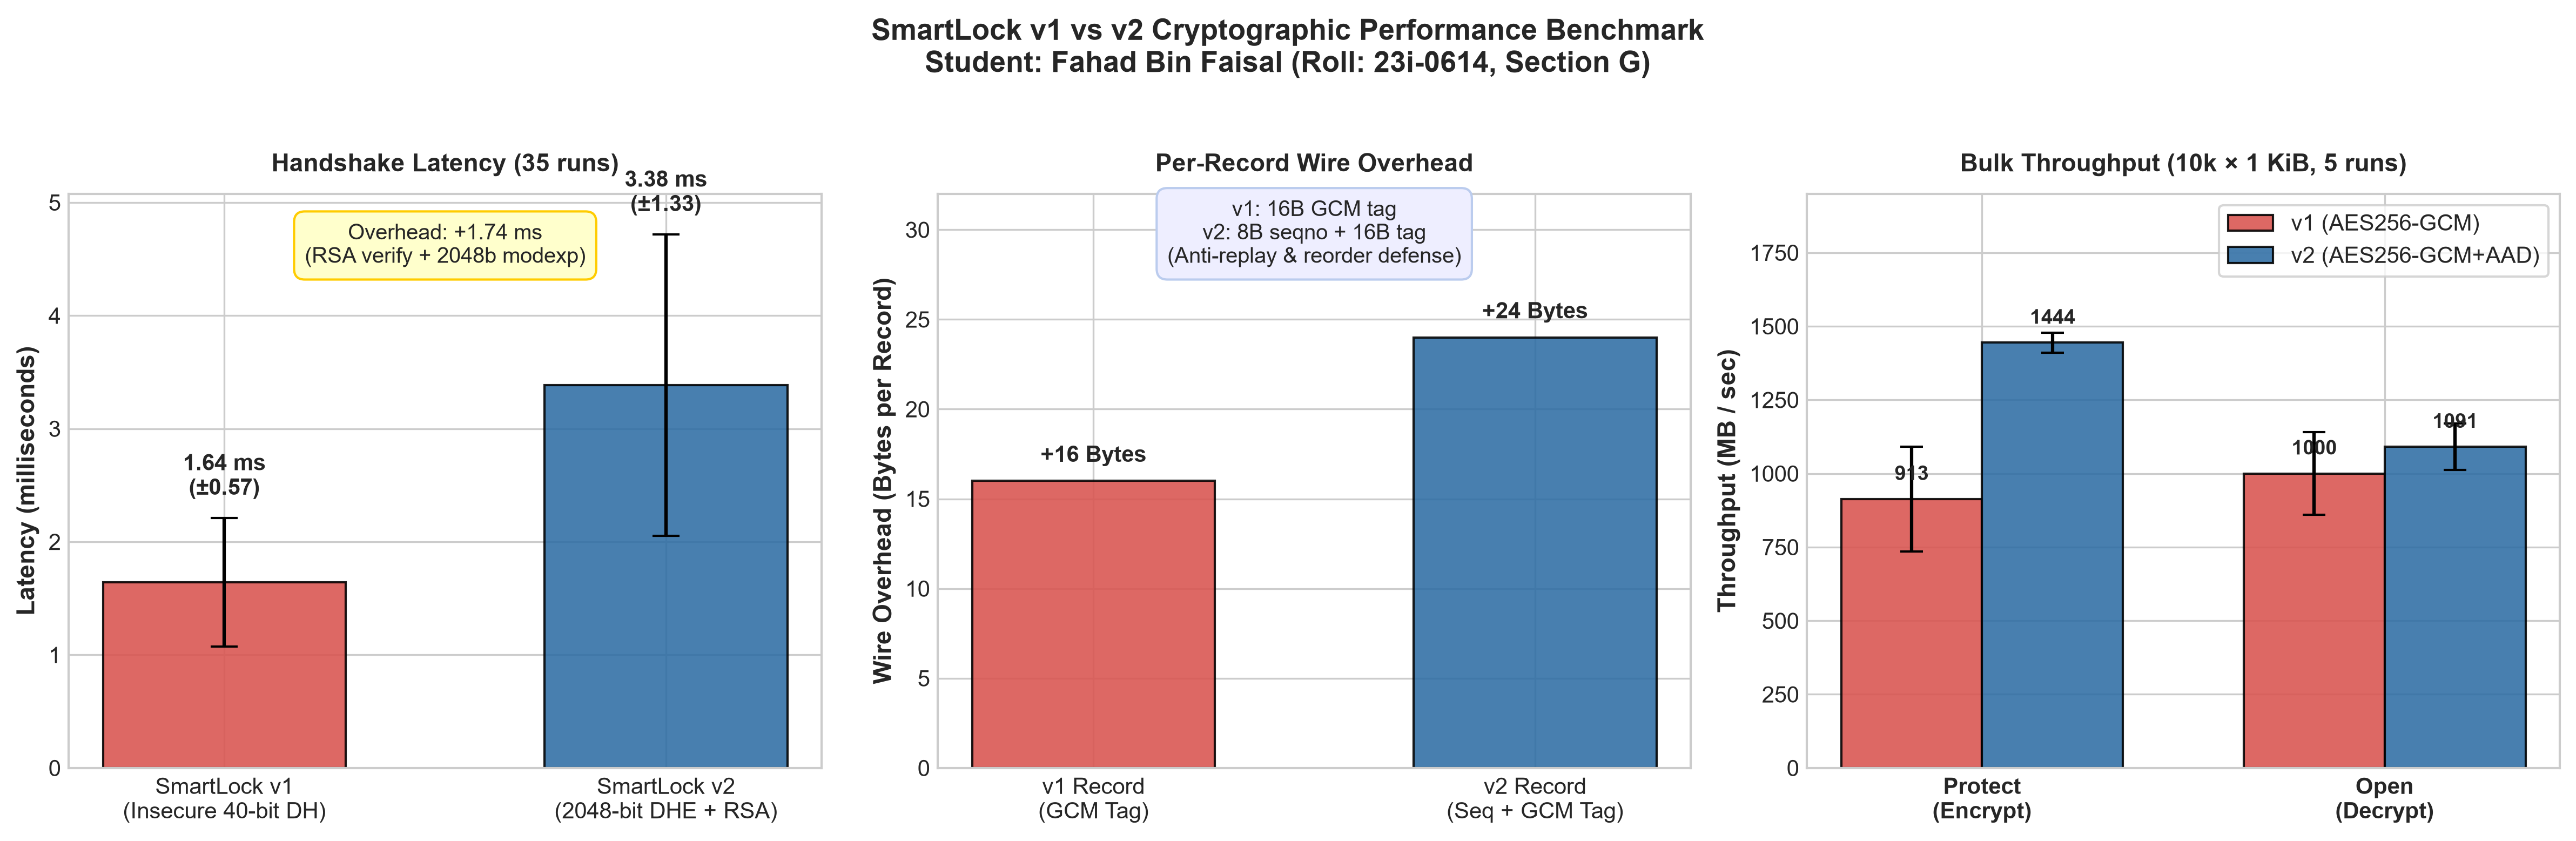
\includegraphics[width=0.98\textwidth]{23i-0614-G/performance/performance_comparison.png}
    \caption{Comparative Cryptographic Benchmark Visualizations (v1 vs v2).}
\end{figure}

\subsection{Engineering Trade-off Defense}
Upgrading from SmartLock v1 to SmartLock v2 increases average handshake latency from $1.64\text{ ms}$ to $3.38\text{ ms}$ ($+1.74\text{ ms}$). This overhead is spent computing 2048-bit modular exponentiations for forward-secure Diffie-Hellman and verifying 2048-bit RSA signatures over the handshake transcript. In an IoT physical door lock, handshakes occur only when a user approaches or an automation session is established. According to established HCI guidelines, response times below $100\text{ ms}$ are perceived as instantaneous by humans. The added latency of $1.74\text{ ms}$ consumes less than $1.8\%$ of this imperceptible threshold, meaning users experience zero perceived lag.

Similarly, adding an 8-byte big-endian sequence counter to each wire frame increases per-record overhead from 16 to 24 bytes. On a standard local Wi-Fi or Ethernet network with an MTU of 1500 bytes, 8 bytes represents less than $0.53\%$ of frame capacity. Per-record cryptographic processing takes only $\approx 0.54\text{ }\mu\text{s}$. Binding this sequence number to the GCM Additional Authenticated Data (AAD) guarantees that any replayed, dropped, or out-of-order packet fails authentication immediately, stopping replay attacks.

Throughput in this benchmark evaluates the raw in-memory cryptographic processing rate of the CPU (in MB/s) using AES-256-GCM hardware acceleration (AES-NI and CLMUL). Both implementations exceed $900\text{--}1400\text{ MB/s}$. Interestingly, SmartLock v2 achieved higher protect throughput ($1444\text{ MB/s}$ vs. $913\text{ MB/s}$) due to optimized memory management: v1's scaffold allocated a separate vector on the heap for the authentication tag and repeatedly invoked \texttt{std::vector::insert}, incurring thousands of heap reallocations and buffer copies. In contrast, v2 pre-allocates the exact wire record buffer once, writing the sequence number, ciphertext, and tag directly into their destination offsets with zero buffer reallocations. Given that physical smart lock commands (\texttt{STATUS}, \texttt{UNLOCK}, \texttt{LOCK}) are tiny ($<64\text{ bytes}$) and infrequent ($<1\text{ message/sec}$), the real-world bandwidth is below $0.1\text{ KB/s}$. Utilizing less than $0.0001\%$ of available cryptographic throughput, SmartLock v2 provides ironclad security without affecting device responsiveness or battery life.

\end{document}
